% !TEX TS-program = pdflatex
% !TEX encoding = UTF-8 Unicode

% This is a simple template for a LaTeX document using the "article" class.
% See "book", "report", "letter" for other types of document.

\documentclass[11pt]{article} % use larger type; default would be 10pt

\usepackage[utf8]{inputenc} % set input encoding (not needed with XeLaTeX)
\usepackage{graphicx}
\usepackage{algorithm}
\usepackage{algorithmicx}
\usepackage{algpseudocode}

%%% Examples of Article customizations
% These packages are optional, depending whether you want the features they provide.
% See the LaTeX Companion or other references for full information.

%%% PAGE DIMENSIONS
\usepackage{geometry} % to change the page dimensions
\geometry{a4paper} % or letterpaper (US) or a5paper or....
% \geometry{margin=2in} % for example, change the margins to 2 inches all round
% \geometry{landscape} % set up the page for landscape
%   read geometry.pdf for detailed page layout information

\usepackage{graphicx} % support the \includegraphics command and options

% \usepackage[parfill]{parskip} % Activate to begin paragraphs with an empty line rather than an indent

%%% PACKAGES
\usepackage{booktabs} % for much better looking tables
\usepackage{array} % for better arrays (eg matrices) in maths
\usepackage{paralist} % very flexible & customisable lists (eg. enumerate/itemize, etc.)
\usepackage{verbatim} % adds environment for commenting out blocks of text & for better verbatim
\usepackage{subfig} % make it possible to include more than one captioned figure/table in a single float
% These packages are all incorporated in the memoir class to one degree or another...

%%% HEADERS & FOOTERS
\usepackage{fancyhdr} % This should be set AFTER setting up the page geometry
\pagestyle{fancy} % options: empty , plain , fancy
\renewcommand{\headrulewidth}{0pt} % customise the layout...
\lhead{}\chead{}\rhead{}
\lfoot{}\cfoot{\thepage}\rfoot{}

%%% SECTION TITLE APPEARANCE
\usepackage{sectsty}
\allsectionsfont{\sffamily\mdseries\upshape} % (See the fntguide.pdf for font help)
% (This matches ConTeXt defaults)

%%% ToC (table of contents) APPEARANCE
\usepackage[nottoc,notlof,notlot]{tocbibind} % Put the bibliography in the ToC
\usepackage[titles,subfigure]{tocloft} % Alter the style of the Table of Contents
\renewcommand{\cftsecfont}{\rmfamily\mdseries\upshape}
\renewcommand{\cftsecpagefont}{\rmfamily\mdseries\upshape} % No bold!

%%% END Article customizations

%%% The "real" document content comes below...

\title{Lab 2: Network Structure}
\author{Ruofan Zhou}
%\date{} % Activate to display a given date or no date (if empty),
         % otherwise the current date is printed 

\begin{document}
\maketitle

\section{Degree Distribution}
After hadoop work and passing the file to the Python script, I got 2 plots as below.
\newline
And the \emph{log-plot looks more useful}, since it persents the property more clearly and we can obviously see a linear relationship on the lower part of the plot;
\newline
We can also see the \emph{nodes with small degress are most frequent}, and \emph{the fraction of highly connected nodes decreases};
\newline
It is like \emph{Exponential Distribution}.
\newline
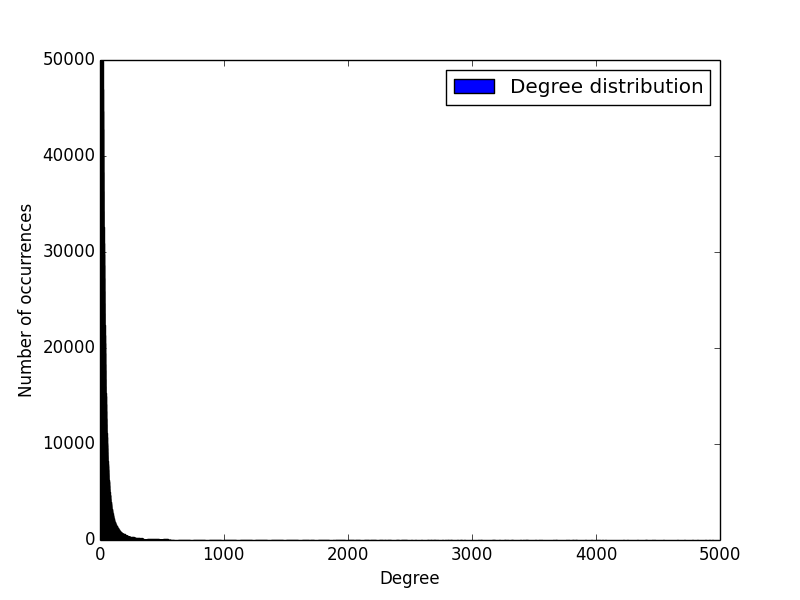
\includegraphics[width=13cm]{pics/degdist-lin}
\\
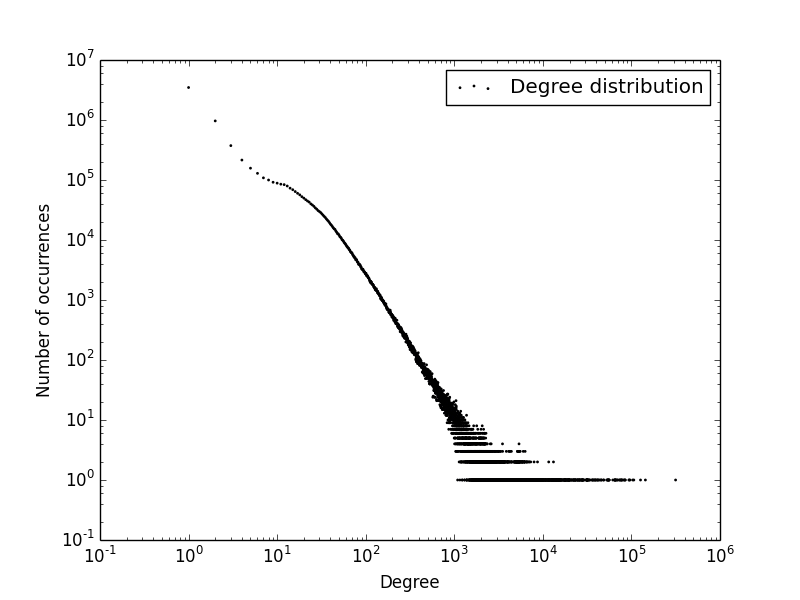
\includegraphics[width=13cm]{pics/degdist-log}

\section{Robustness of Giant Componet}
See file \emph{TargetedRemoval.java} to view my implementation of the class. And here's the pseudo-code of the algorithm:
\\
\begin{algorithm}
	\begin{algorithmic}[1]
		\Function {apply}{$graph$}
			\State $originalSize \gets graph.GCsize()$
			\While {$graph.GCsize > originalSize * 0.2$}
				\State $removeSum \gets 0$
				\While {There exists Edges E=(a,b) such that the removal of E makes the distance of a and b larger than 2}
					\State remove E
					\State $removeSum \gets removeSum + 1$
				\EndWhile
				\While {$removeSum < 100$}
					\State randomly remove a edge E
					\State $removeSum \gets removeSum + 1$
				\EndWhile
			\EndWhile
		\EndFunction
	\end{algorithmic}
\end{algorithm}
\\
The Random algorithm uses 121,000 removals, and 92,000 for TragetedRemoval algorithm. See plot as below:
\\
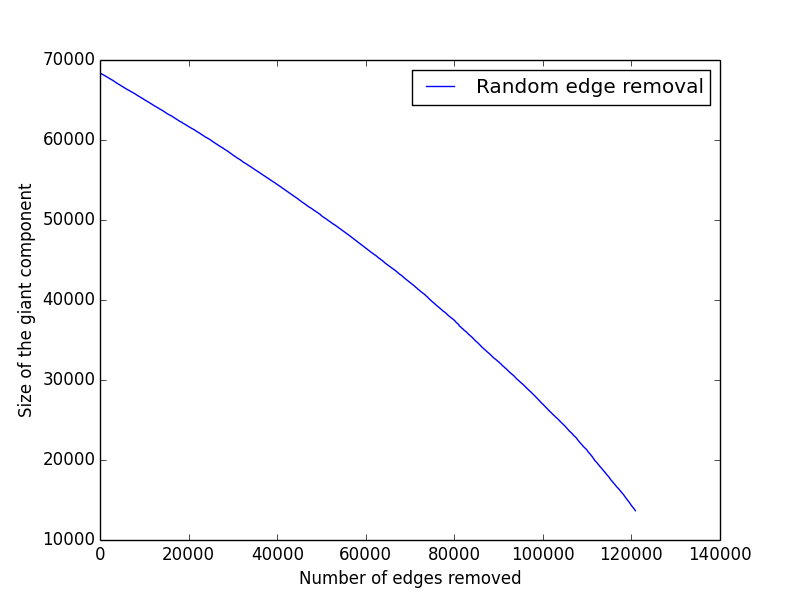
\includegraphics[width=13cm]{pics/giant-component-1}
\\
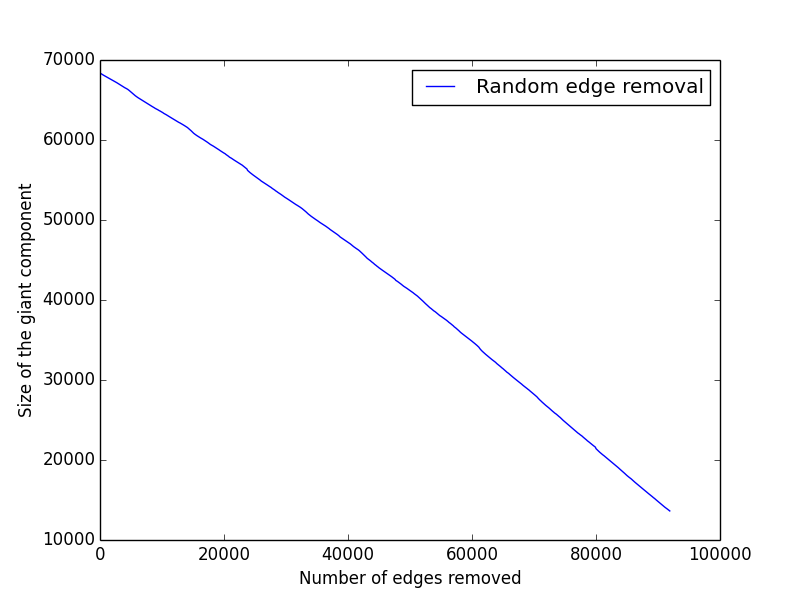
\includegraphics[width=13cm]{pics/giant-component}

\end{document}
